% Chapter 1

\chapter{Hierarchical Deterministic Wallet} % Main chapter title

\label{hd wallet} % For referencing the chapter elsewhere, use \ref{Chapter1}

%----------------------------------------------------------------------------------------

% Define some commands to keep the formatting separated from the content 
%\newcommand{\keyword}[1]{\textbf{#1}}
%\newcommand{\tabhead}[1]{\textbf{#1}}
%\newcommand{\code}[1]{\texttt{#1}}
%\newcommand{\file}[1]{\texttt{\bfseries#1}}
%\newcommand{\option}[1]{\texttt{\itshape#1}}

%----------------------------------------------------------------------------------------

In this chapter we will see how an HD wallet works.

\section{Elements}
Let's focus on the main elements of the Wallet:
\begin{itemize}[label=$\diamond$]
	\item Seed
	\item Extended keys
\end{itemize}

\subsection{Seed}
The entire Wallet is based on a \textit{seed}.
\\ \\
It is a number taken from a \textit{Discrete Uniform Random Variable}
\begin{equation*}
seed=X(\omega) \qquad X\sim \mathcal{U}(S)
\end{equation*}
Where $S$ is the finite set of natural number in the range from $1$ to an arbitrary value.\\ Obviously the greater the set from which the number can be extracted, the better it is for the security of the seed itself.
\\ \\
This is an example of seed expressed in hexadecimal format: \\
\textit{seed}=fffcf9f6f3f0edeae7e4e1dedbd8d5d2cfccc9c6c3c0bdbab7b4b1aeaba8a5a29f9c999 \\ 693908d8a8784817e7b7875726f6c696663605d5a5754514e4b484542 

\subsection{Extended Key}
An Extended Key is a sequence of bytes, encoded in base58. It contains all the information necessary derive the keys. When the derivation is made for the first time from the seed, the extended key is called master key.\\ \\
Once it is decoded we will obtain exactly 78 bytes, with a specific meaning and order:
\begin{itemize}[label=$\circledast$]
	\item 4 bytes are used to specified the \textbf{version}.
	\item 1 byte is used to specified the \textbf{depth} in the hierarchical tree: the extended key derived directly from the seed has $depth=0$, its first children have $depth=1$, grandchildren have $depth=2$ and so on.
	\item 4 bytes are used for the \textbf{fingerprint}. It is a unique value that identify the parent. Compute the HASH160 function on the "parent" public key in a compressed form and then take the first 4 bytes:
	\begin{equation*}
	fingerprint=HASH160(\text{parent public key})[0:4]
	\end{equation*}
	Where $[0:4]$ is a python notation.\\
	For the master key the fingerprint is formed by 4 zeros bytes: $fingerprint=0000000000$
	\item 4 bytes are used to specified the \textbf{index} of the child. \\
	For the master key the index is formed by 4 zeros bytes: $index=0000000000$
	\item 32 bytes are used for the \textbf{chain code}. The chain code is used in order to introduce entropy in the children generation. We will see below how it works.
	\item 33 bytes are used for the \textbf{key}. It can be \textit{private} or \textit{public}. \\ Public key is expressed in compress form, so the first byte is always $02$ or $03$. The first byte of the private key is always $00$ in order to distinguish the key from the public one.\\
\end{itemize}
An extended key is called \textbf{Extended Private Key} if the lasts 33 bytes are used to specify the private key; it is called \textbf{Extended Public Key} if they are used to specify the public key.
\\ \\
For the Bitcoin mainnet it is used for the \textbf{version}: $0x0488ADE4$ for an extended private key, $0x0488B21E$ for an extended public key. When this bytes are encoded in base58, they returns \textit{xprv} and \textit{xpub} respectively.

\begin{remark}
	Obviously it is possible to calculate the extended public key starting from the extended private key, but it is infeasible to do the opposite. The only difference between the two extended keys are the \textbf{key bytes} and the \textbf{version bytes}, all the others elements remain the same.
\end{remark}

\section{From SEED to Master Private Key}
In this section we will see in detail how it is possible to switch from a \textit{seed} to a \textit{master private key}. \\ \\
First of all we need to convert the seed into a string of bytes, where the most significant bytes come first (big endian). In order to do so, we need to know the length of the string of bytes. \\ \\
Let's see a practical example:
\begin{equation*}
\begin{split}
&byte\_string_1=00\; 00\; 00 \; 01 \\
&byte\_string_2=00\; 00\; 01 \\
&byte\_string_3=00\; 01 \\
&byte\_string_4=01
\end{split}
\end{equation*}
These $4$ byte strings are obtained from the same seed: $seed=1$ and the only different is the length of the string.
\begin{remark}
	Different length of string produce different master private key, even if the seed is the same number.
\end{remark}
In python:
\begin{lstlisting}[language=Python]
byte_string = seed.to_bytes(seed_bytes, 'big')
\end{lstlisting}
Where $seed$ is an integer number, \textit{seed\_bytes} is the number of bytes that the \textit{byte\_string} should have. 
\\ \\
It is essential to specify the length of the byte string, otherwise there will be obtained different wallets. \\ \\
Once we obtain a string of bytes, we will compute the HMAC algorithm. The hash function used for HMAC is the SHA512 and the \textit{key} is a particular string of bytes: \textit{b"Bitcoin seed"}. In python the implementation is the follow:

\begin{lstlisting}[language=Python]
from hashlib import sha512
from hmac import HMAC

hashValue = HMAC(b"Bitcoin seed", byte_string, sha512).digest()
\end{lstlisting}
Where \textit{.digest()} is used in order to return a string of bytes.
\\ \\
Now we have obtained an \textit{hashValue} of $512$ bits, so $64$ bytes. Consider the firsts $32$ bytes as the master private key and the next $32$ bytes as the master chain code. A python implementation is the follow:

\begin{lstlisting}[language=Python]
private_key_bytes = hashValue[0:32]
chain_code_bytes = hashValue[32:64]
\end{lstlisting}
\begin{flushleft}
	Now we have two byte strings, one for the master private key and the other for the master chain code.
\end{flushleft}
It is important to remember that a private key must be in the range between $1$ and $order$, so the byte string for the private key should be converted in \textit{int} and then take the \textit{mod order}. In python we have:

\begin{lstlisting}[language=Python]
private_key = int(private_key_bytes.hex(), 16) % order
\end{lstlisting}
\begin{flushleft}
	Finally we will concatenate all the informations obtained in order to form a Master Extended Private Key (in bytes format):
\end{flushleft}

\begin{itemize}
	\item vbytes = $b'\backslash x04\backslash x88\backslash xAD\backslash xE4'$
	\item depth = $b'\backslash x00'$
	\item fingerprint = $b'\backslash x00\backslash x00\backslash x00\backslash x00'$
	\item index = $b'\backslash x00\backslash x00\backslash x00\backslash x00'$
	\item chain code is the one previously computed
	\item private key = $b'\backslash x00'$ $+$ private key in bytes format, previously computed.
\end{itemize}
Then the Master Extended Private Key is formed by concatenation:

\begin{lstlisting}[language=Python]
xkey = vbytes + depth + fingerprint + index + chain_code + key
\end{lstlisting}
\begin{flushleft}
	In order to make it readable, a base58 encode is performed.
\end{flushleft}
This is an example of Master Extended Private Key: \\
xprv9s21ZrQH143K3wEaiSJZ8jYCuZF1oJoXHiwFcx2WwXqQHD4ZLdyEAFZ22M4 BmQT82HRbWssLArj53YDQTj6vSN4iH6nTiSQ61C5CckxUtDq

\begin{remark}
	The SHA512 is an irreversible function, so it is infeasible to obtained the seed, knowing the Extended Key. (It is also useless because with the master key you can derive all the keys in the wallet).
\end{remark}

\begin{flushleft}
	Graphically these operation can be shown in figure \ref{fig:From seed to master private key}
\end{flushleft}

\begin{figure}[ht!]
	\centering
	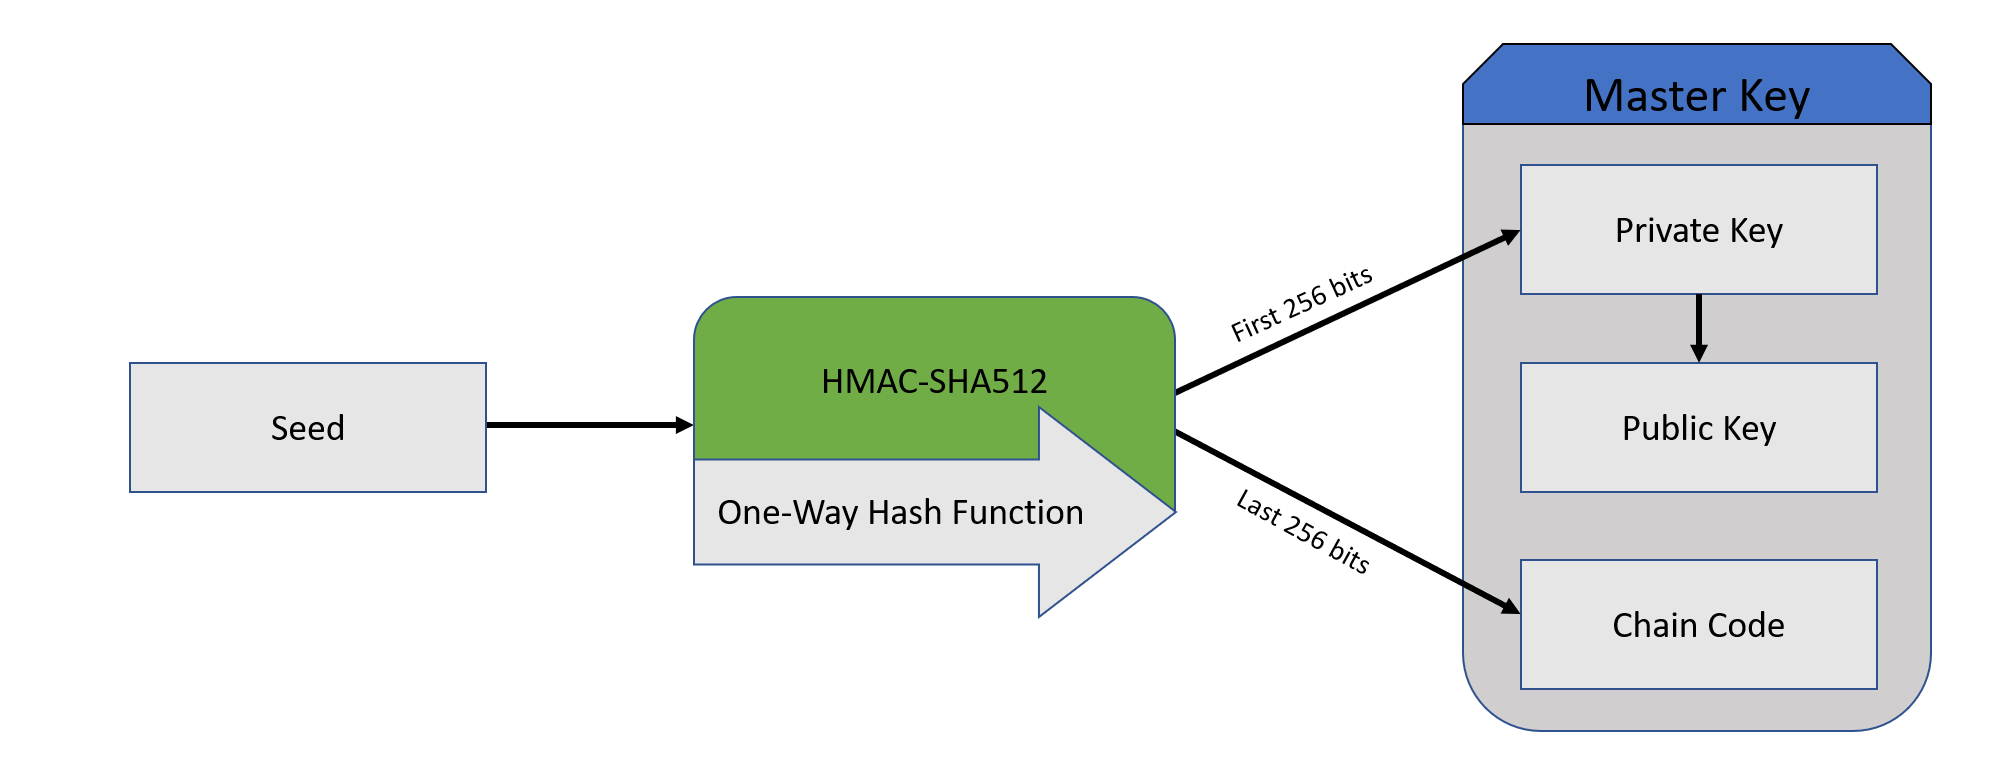
\includegraphics[width=14.5cm]{Figures/seed_to_xprv_v2.png}
	\caption{From seed to master private key}
	\label{fig:From seed to master private key}
\end{figure}


\section{Child Key derivation}
From any extended private key it is possible to obtain different child keys. There are two method used in order to do so:
\begin{itemize}
	\item Normal
	\item Hardened
\end{itemize}
Both methods have some advantage and disadvantage that we will discuss later. For every situation it is essential to use the method that best fit.
\\ \\
For both the method the derivation starts from an extended private key. From this key some essential information are necessary:
\begin{itemize}[label=$\star$]
	\item Chain code
	\item Private key
\end{itemize}
It is also required a number, used in order to specify the \textbf{index} of the child. This number should be in the range between $0$ and $4294967295$. This is due to the fact that in any Extended Key there are 4 bytes used to specify the index of the child:
\begin{equation*}
max \; index=(FF\;FF\;FF\;FF)_{base \; 16} = 2^{32} = 4294967295
\end{equation*}
In fact it is possible to generate even a greater number of children from the same parent, but it would not be possible to write the corresponding Extended Key in the format described above.


\subsection{Normal derivation}

First we need to compute the Parent Public Key $P$. This is obtained from the usual scalar multiplication between a point on the EC (the Generator $G$) and the Parent Private Key $p$:

\begin{equation*}
P=p\cdot G
\end{equation*}
Consider only the compress form of $P$ and convert this value into a byte string, obtaining 33 bytes.
\\ \\
Concatenate this 33 byte string to the 4 byte string representing the index number:

\begin{equation*}
msg = compressed \; public\;key \;|\; index
\end{equation*}
$msg$ is a string of $37$ bytes. \\ \\
Apply the HMAC algorithm with the following input:

\begin{itemize}[label=$\odot$]
	\item \textbf{Hash function}: SHA512
	\item \textbf{Key}: chain code
	\item \textbf{Message}: $msg$
\end{itemize}
The Python code is the follow:
\begin{lstlisting}[language=Python]
from hmac import HMAC
from hashlib import sha512

msg=parent_public_key + index
hashValue = HMAC(parent_chain_code, msg, sha512).digest()
\end{lstlisting}
\begin{flushleft}
	The result is a string of 64 bytes: \textit{hashValue}.
\end{flushleft}
Split this string of bytes in two: the last 32 are the child chain code. Take the first 32 bytes, convert them into an integer number and sum it to the parent private key (mod \textit{order}), obtaining the child private key.\\ \\
This is the python code:

\begin{lstlisting}[language=Python]
child_chain_code = hashValue[32:]
q = int(hashValue[:32].hex(), 16)
child_private_key = (q + parent_private_key) % order
\end{lstlisting}

\begin{flushleft}
	Graphically these operation can be shown in figure \ref{fig:normal_derivation}
\end{flushleft}

\begin{figure}[ht!]
	\centering
	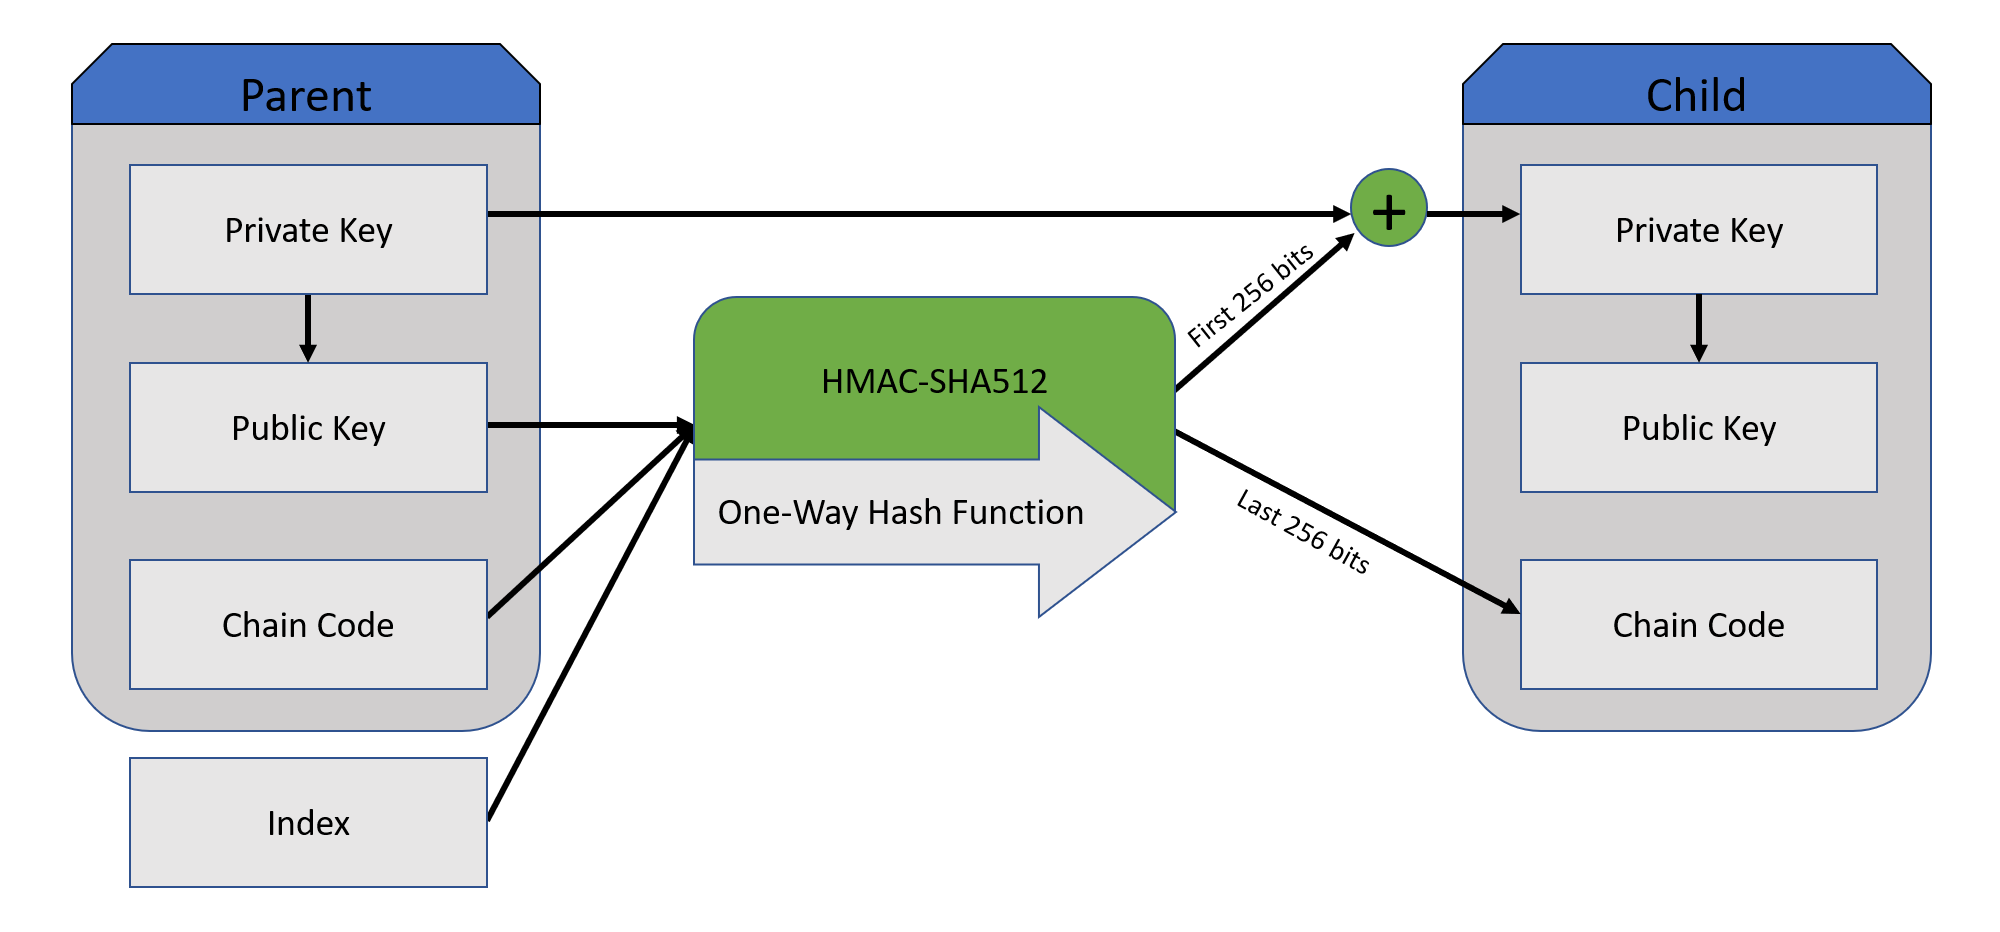
\includegraphics[width=14.5cm]{Figures/normal_derivation_v2.png}
	\caption{Normal Derivation }
	\label{fig:normal_derivation}
\end{figure}


\subsection{Hardened derivation}
This method is similar to the previous one, the only difference is that as input of the \textit{hash} function the private key is used instead of the public one. \\ \\
Concatenate the 33 bytes of parent private key, considering also the $00$ byte, with the 4 byte string representing the index number:

\begin{remark}
In order to better distinguish the hardened derivation from the normal one, the numbering of the indices starts from the number $2^{31}.$
\end{remark} 
\begin{equation*}
msg = 00 \;|\; private\;key \;|\; index
\end{equation*}
$msg$ is a string of $37$ bytes. \\ \\
Apply the HMAC algorithm with the following input:

\begin{itemize}[label=$\odot$]
	\item \textbf{Hash function}: SHA512
	\item \textbf{Key}: chain code
	\item \textbf{Message}: $msg$
\end{itemize}
The Python code is the follow:
\begin{lstlisting}[language=Python]
from hmac import HMAC
from hashlib import sha512

msg=parent_private_key + index
hashValue = HMAC(parent_chain_code, msg, sha512).digest()
\end{lstlisting}
\begin{flushleft}
	The result is a string of 64 bytes: \textit{hashValue}. In this code the $parent\_private\_key$ already has the first $00$ byte, because it is taken directly from the parent extended private key.
\end{flushleft}
Split this string of bytes in two (in the same way as the normal method): the last 32 are the child chain code. Take the first 32 bytes, convert them into an integer number and sum it to the parent private key (mod \textit{order}), obtaining the child private key.\\ \\
This is the python code:

\begin{lstlisting}[language=Python]
child_chain_code = hashValue[32:]
q = int(hashValue[:32].hex(), 16)
child_private_key = (q + parent_private_key) % order
\end{lstlisting}


\begin{flushleft}
	Graphically these operation can be shown in figure \ref{fig:hardened_derivation}
\end{flushleft}

\begin{figure}[ht!]
	\centering
	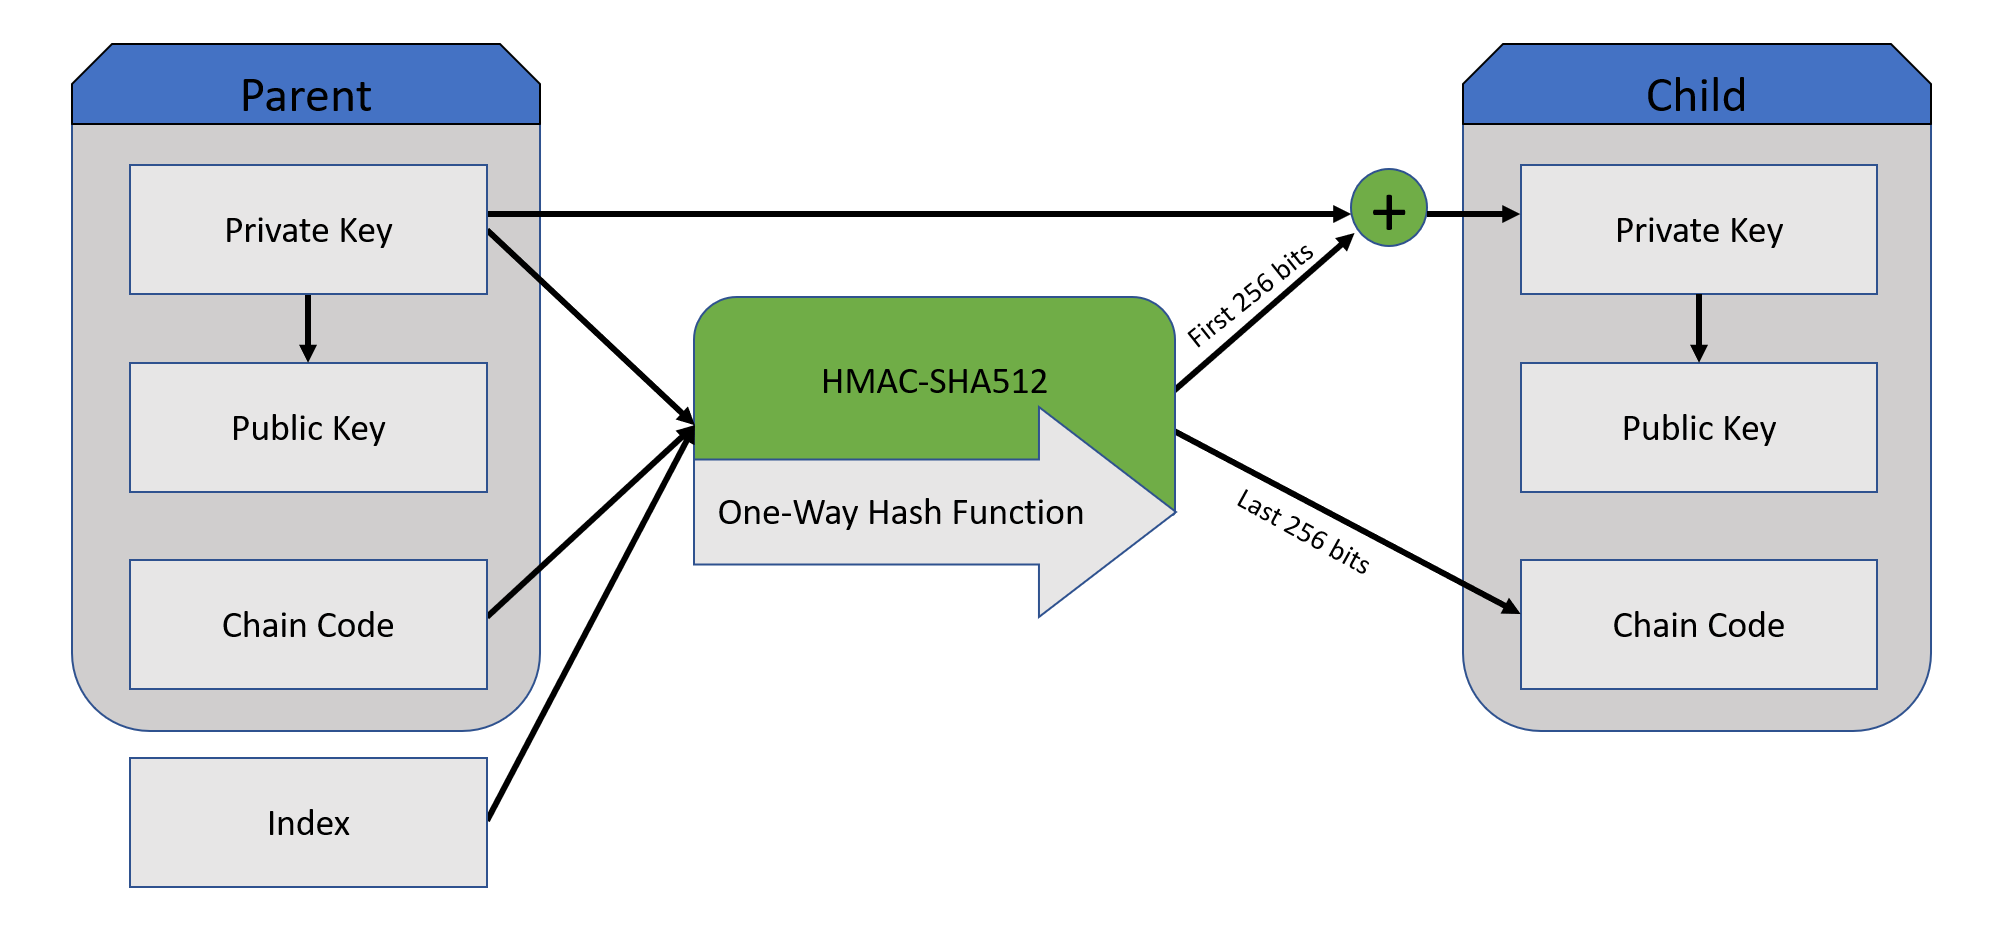
\includegraphics[width=14.5cm]{Figures/hardened_derivation_v2.png}
	\caption{Hardened Derivation }
	\label{fig:hardened_derivation}
\end{figure}


\section{Special derivation}
Using a \textit{normal derivation} it is possible to derive the extended public key, starting only from the extended public key of the parent.

\subsection{Public derivation}

In order to compute this particular derivation, the only essential elements are the ones contained in the extended public key, in particular:

\begin{itemize}
	\item Public key $P_{parent}$
	\item Chain code
	\item Index
\end{itemize}
First apply the HMAC algorithm to the same input used for the normal derivation:
\\ \\
Concatenate the 33 byte string of the public key to the 4 byte string representing the index number:

\begin{equation*}
msg = compressed \; public\;key \;|\; index
\end{equation*}
Apply the HMAC algorithm with the following input:

\begin{itemize}[label=$\odot$]
	\item \textbf{Hash function}: SHA512
	\item \textbf{Key}: chain code
	\item \textbf{Message}: $msg$
\end{itemize}
The output of this function is the same of the normal derivation with the extended private key. The last 32 bytes formed the child chain code, instead the first 32 bytes can be read as a special number: $q$. \\ \\
Multiply the generator $G$ to the integer number $q$ and obtain $Q$, a point on the EC:
\begin{equation*}
Q=q\cdot G
\end{equation*}
Compute the sum between two point on the elliptic curve: $Q$ and $P_{parent}$, where $P_{parent}$ is the parent public key.
\begin{equation*}
Q+P_{parent}=P_{child}
\end{equation*}
Where $P_{child}$ is the child public key. 
\\ \\
We will now prove that the child public key obtained in this way $P_{child_2}$ is the same as that obtained starting from the private key, $P_{child_1}$:
\\ \\
Both the procedures start from $q$, number obtained from the first 32 bytes of the HMAC function. Let's call $p_{parent}$ the parent private key and $p_{child}$ the child private key.

\begin{equation*} \label{eq2}
\begin{split}
P_{child_1} & = p_{child} \cdot G \\
& = (q+p_{parent}) \cdot G \\
& = (q \cdot G) + (p_{parent}\cdot G) \\
& = Q + P_{parent} = P_{child_2}
\end{split}
\end{equation*}
\begin{flushright}
	\textit{cvd}
\end{flushright}
Graphically this derivation can be shown in figure \ref{fig:pubtopub}
\begin{figure}[ht!]
	\centering
	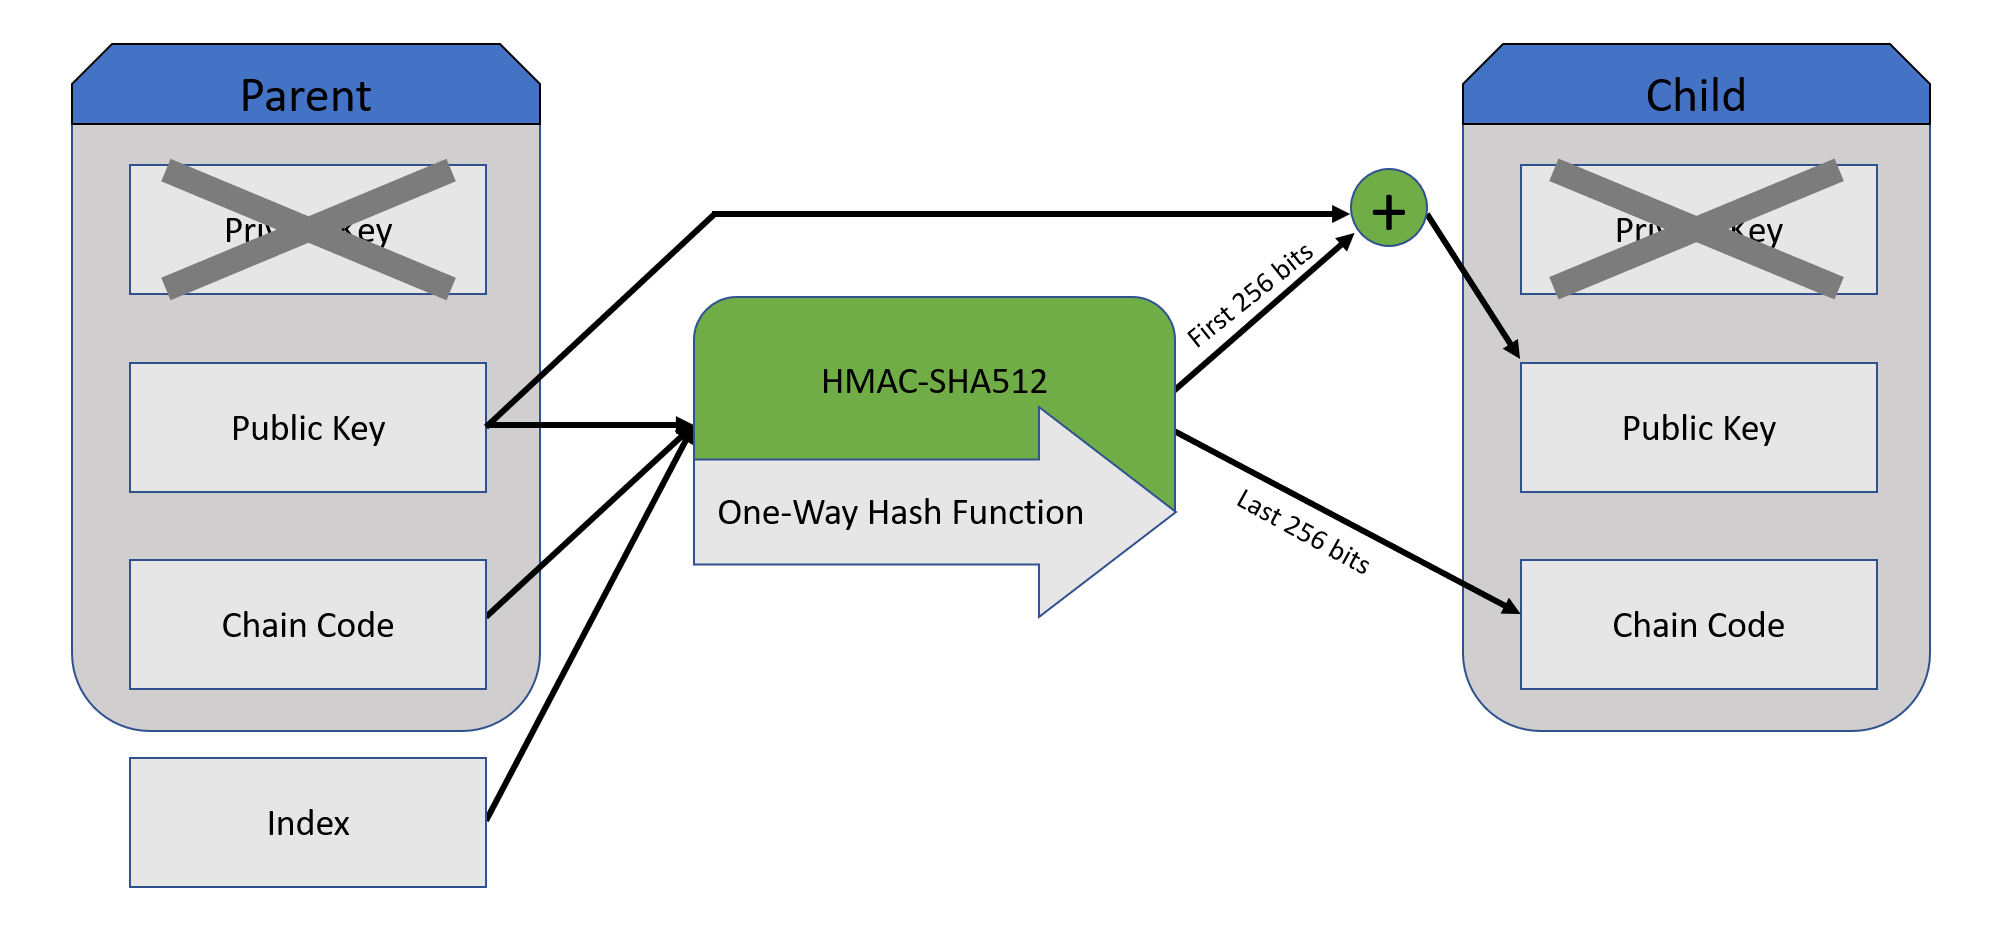
\includegraphics[width=14.5cm]{Figures/pubtopub.png} %cambiare immagine
	\caption{Public Derivation}
	\label{fig:pubtopub}
\end{figure}

\subsection{Weakness of Normal Derivation}
As shown above the normal derivation present a great advantage, but also a weakness. It is possible to derive the \textbf{parent extended private key} knowing the \textbf{parent extended public key} and only one of the \textbf{child extended private key}.
\\ \\
The HMAC-SHA256 function has as input three elements: the parent chain code, the parent public key and the child index. The firsts two information can be taken from the parent extended public key, instead the child index can be taken from the child extended private key.

\begin{equation*}
msg = compressed \;parent\; public\;key \;|\;child\; index
\end{equation*}
Then apply the HMAC algorithm with the usual input:

\begin{itemize}[label=$\odot$]
	\item \textbf{Hash function}: SHA512
	\item \textbf{Key}: parent chain code
	\item \textbf{Message}: $msg$
\end{itemize}
Consider the first 32 bytes of the result of this function and consider it as an integer number, $q$.
\\ \\
Remembering that to get the child private key it is needed to compute a sum with the parent private key, it is possible to reverse the process. \\ \\
Let's call $p_{child}$ and $p_{parent}$ the private keys of the child and the father respectively.
\begin{equation}\label{eq3}
\begin{split}
p_{child} &= q+p_{parent} \qquad \mod (order) \\
&\Downarrow \\
p_{parent} &=p_{child}-q \qquad \mod (order)
\end{split}
\end{equation}
The implication \ref{eq3} holds also with modular arithmetic.
\\ \\
So we have derived the private key of the parent. Graphically this derivation can be shown in figure \ref{fig:from_child_to_parent}
\begin{figure}[ht!]
	\centering
	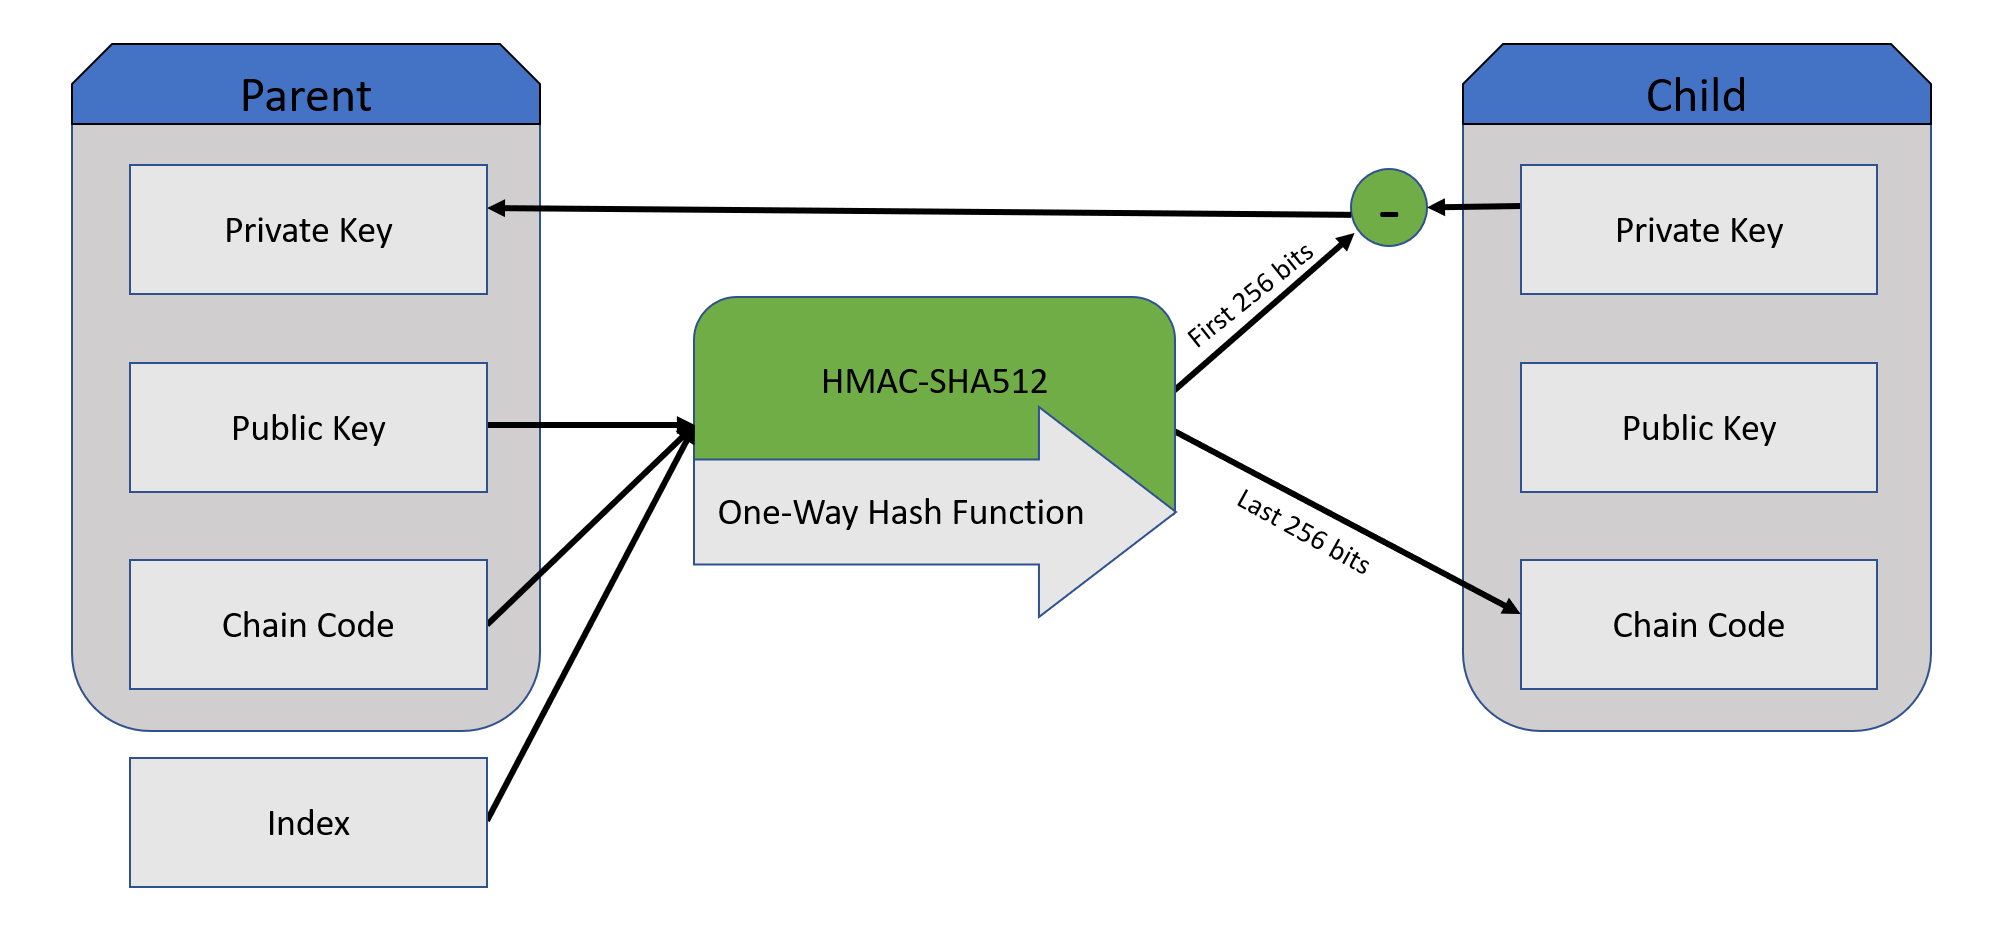
\includegraphics[width=14.5cm]{Figures/childtoparent.png} %cambiare immagine
	\caption{From child to parent}
	\label{fig:from_child_to_parent}
\end{figure}



\section{Advantages and disadvantages}
We have seen that public-to-public operation is possible using the normal derivation. This is impossible with the hardened one: \\ \\
The input of HMAC-SHA512 are different for the two derivation. If for the normal derivation is sufficient only the information in the public extended key, for the hardened derivation, the parent private key is needed. This makes impossible to obtain a public from a public, but also it makes impossible to derive the private key of the parent knowing the private key of the child and the public of the parent.
\\ \\
Knowing strengths and weaknesses of the two methods, it is advisable to use each of the two methods in the appropriate situations.

\subsection{When use Normal Derivation?}
Normal derivation should be used whenever all the child keys are collected in the same digital place and you should never give one key to someone else. As already mention a leak of a single private key can compromise the entire wallet.
\\ \\
However if all the child keys are used by the same person and you need to generate different public key, with this derivation it is possible to do so even in a "hot place". Let's suppose to have stored only the extended public key in a device, you can then receive payment to yours public keys, but it is impossible to spend those coins as long as the private keys are hidden. If someone stole your device the only problem is a leak of privacy, because it is possible, by examining the blockchain, to discover all the UTXOs associated with that wallet.


\subsection{When use Hardened Derivation?}
Hardened derivation should be used whenever all the keys generated are used for different purpose or are stored in different places. With this procedure it is possible to yield a branch of the tree to someone else in order to manage part of your money, without the risk to lose all the others keys in the wallet.
\\ \\
As a best practice it is always advisable to derive with the hardened method from the master. An hardened key should have both hardened or normal children, but from a normal child it is not reasonable to derive an hardened one, because it make no sense to increase the security of the wallet at the last level.


